\documentclass{article}%
\usepackage[T1]{fontenc}%
\usepackage[utf8]{inputenc}%
\usepackage{lmodern}%
\usepackage{textcomp}%
\usepackage{lastpage}%
\usepackage[head=40pt,margin=0.5in,bottom=0.6in]{geometry}%
\usepackage{graphicx}%
%
\title{\textbf{Regreso de Guaidó a Venezuela: qué se juega el oficialismo y la oposición}}%
\author{NO\_TIENE}%
\date{04/03/2019}%
%
\begin{document}%
\normalsize%
\maketitle%
\textbf{URL: }%
http://www.el{-}nacional.com/noticias/bbc{-}mundo/regreso{-}guaido{-}venezuela{-}que{-}juega{-}oficialismo{-}oposicion\_273306\newline%
%
\textbf{Periodico: }%
EN, %
ID: %
273306, %
Seccion: %
BBC Mundo\newline%
%
\textbf{Palabras Claves: }%
Nicolás Maduro, Juan Guaidó\newline%
%
\textbf{Derecho: }%
2.1%
, Otros Derechos: %
\newline%
%
\textbf{\textit{El líder opositor retorna a Venezuela para encabezar una serie de movilizaciones en contra de Nicolás Maduro, pero corre el riesgo de ser detenido por violar una prohibición de salida del país emitida por el Tribunal Supremo de Justicia}}%
\newline%
\newline%
%
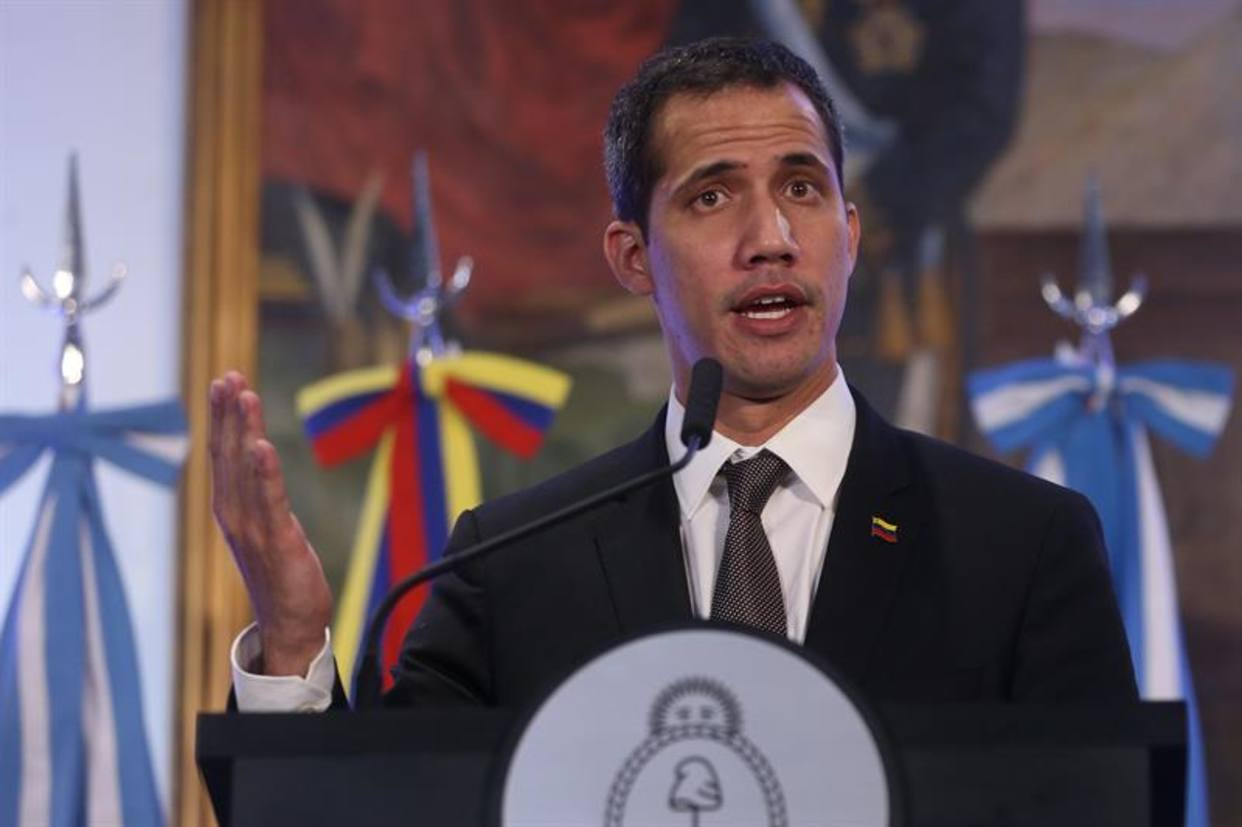
\includegraphics[width=300px]{EN_273306.jpg}%
\newline%
%
"Anuncio mi regreso al país y la convocatoria de movilizaciones en todo el territorio nacional para este lunes y martes".%
\newline%
%
Con esas palabras publicadas en Twitter, el presidente de la Asamblea Nacional de Venezuela, Juan Guaidó, puso fin el sábado a las dudas sobre su intención de retornar a su país, donde~corre el riesgo de ser enviado a prisión.%
\newline%
%
El diputado opositor se juramentó como presidente interino~de la República el pasado 23 de enero, prometiendo conducir un gobierno de transición que convoque elecciones libres argumentando que Nicolás Maduro~estaba usurpando el poder por haber sido electo en unos comicios fraudulentos.%
\newline%
%
Su actuación valió para que Maduro le acusara de intentar dar un golpe de Estado y para que el Tribunal Supremo de Justicia dictara en su contra una~orden de prohibición de salida del país.%
\newline%
%
Guaidó desafió esa restricción abiertamente al viajar a Colombia para asistir a una cumbre del Grupo de Lima y, posteriormente, visitar Paraguay, Brasil, Argentina y Ecuador.%
\newline%
%
La respuesta del oficialismo no se hizo esperar.~Maduro anunció que el líder opositor deberá rendir cuentas ante el Poder Judicial.~"Él no puede ir y venir\&mldr; y la justicia le tenía prohibido dejar el país. Yo respeto las leyes", dijo.%
\newline%
%
Maduro dijo que Guaidó debe someterse a la ley| GETTY IMAGES%
\newline%
%
Por su parte, Diosdado Cabello, el número dos del chavismo gobernante, aseguró en tono amenazante~que las autoridades estarían aguardando a Guaidó.%
\newline%
%
"Ahí lo estamos esperando. Jorge~García Carneiro le tiene un comité de recepción", dijo Cabello haciendo mención al gobernador del estado Vargas, donde se ubica el Aeropuerto Internacional de Maiquetía, principal puerto de entrada de vuelos internacionales a Venezuela.%
\newline%
%
Tensando la cuerda%
\newline%
%
En un mensaje difundido este domingo en directo a través de sus cuentas en redes sociales, Guaidó confirmó su regreso a Venezuela para encabezar las manifestaciones convocadas para este lunes a las 11:00 am, hora local.%
\newline%
%
"Mañana lunes~tenemos un reto histórico. Regresamos a nuestro país", dijo el dirigente venezolano desde un lugar no identificado.%
\newline%
%
¿Pero, qué se juegan oficialismo y oposición con esta vuelta de Guaidó a Venezuela?%
\newline%
%
Guaidó retorna después de que el 23 de febrero la oposición no logró hacer ingresar la ayuda humanitaria donada por Estados Unidos y otros países para atender a decenas de miles de venezolanos.%
\newline%
%
El oficialismo bloqueó el paso por las fronteras de Venezuelacon Colombia, Brasil~y con las islas caribeñas de~Aruba, Curazao y Bonaire.%
\newline%
%
En algunos casos, la entrada de la ayuda fue impedida con un fuerte uso de la fuerza que causó varios muertos y más de 60 heridos de bala, según la ONG venezolana Foro Penal.%
\newline%
%
Esa represión fue duramente criticada por el~Grupo de Lima~{-}formado por aliados de Guaidó{-} que, sin embargo, descartó usar la fuerza militar para lograr un cambio político en Venezuela.%
\newline%
%
Parte de la ayuda humanitaria se perdió en las confrontaciones en la frontera de Venezuela con Colombia| EPA%
\newline%
%
Poco después, Elliot Abrams, el funcionario nombrado por Donald Trump para hacer frente a la crisis venezolana, dijo que~Estados Unidos respondería de forma política y diplomática~a una eventual detención de Guaidó por parte de Maduro.%
\newline%
%
Estas reacciones fueron consideradas por algunos analistas como reveses para la oposición y llevaron a dudar sobre si el dirigente venezolano se atrevería a regresar a su país en esas circunstancias.%
\newline%
%
Carmen Beatriz Fernández, consultora política venezolana, directora de Datastrategia y profesora invitada de la Universidad de Navarra, considera que el retorno del dirigente es muy importante.%
\newline%
%
"Guaidó es mucho más útil para la oposición como presidente encargado dentro de Venezuela que en el exilio.~Lo contrario habría sido probablemente un baño de agua fría para los venezolanos", señala.%
\newline%
%
Asegura que la sociedad venezolana se encontraba "en una situación de depresión social y políticamente se sentía como si el régimen había logrado quebrarle las ganas de rebelarse" y que con la aparición de Guaidó en la escena desde inicios de enero, esa situación cambió de la noche a la mañana.%
\newline%
%
"El regreso de Guaidó a Venezuela está forzando la barra (tensando la cuerda) en los dos sentidos: pone al gobierno en una disyuntiva perder{-}perder", afirma la experta.%
\newline%
%
Advierte que~si Maduro detiene al opositor puede enfrentar una dura respuesta internacional, pero si lo deja libre, quedará muy debilitado ante los mismos factores que le apoyan.%
\newline%
%
Ante este dilema, Fernández cree que desde el punto de vista del gobierno la respuesta más lógica es tratar de detener a Guaidó.%
\newline%
%
Ángel Álvarez, politólogo venezolano y consultor en Políticas Públicas de organizaciones internacionales, cree que la importancia del regreso de Guaidó a Venezuela depende del éxito que tenga en su empeño.%
\newline%
%
"Si se estima que al hacerlo puede ser detenido indefinidamente y eso no contribuye sino a la consolidación de Maduro, evidentemente para él no va a ser conveniente regresar. Por otra parte, si permanecía en el exterior podía ser visto como eludiendo sus responsabilidades", apunta.%
\newline%
%
Escenarios%
\newline%
%
Álvarez considera que el peor escenario para Guaidó sería uno en el que fuese~detenido y aislado de sus bases de apoyo y de la comunidad internacional, y que termine en circunstancias parecidas a las del dirigente venezolano Leopoldo López.%
\newline%
%
El dirigente de Voluntad Popular, en el que milita Guaidó, está privado de su libertad desde 2014 y, pese a que en la actualidad está en arresto domiciliario, no puede participar abiertamente en política.%
\newline%
%
"Es lo peor que le podría ocurrir porque~podría producir desmovilización y desgaste", señala.%
\newline%
%
Un segundo escenario sería que Maduro perciba que no puede detener al opositor porque correría el riesgo de provocar reacciones internacionales muy importantes así como fuertes respuestas internas.%
\newline%
%
"En ese caso, Maduro perdería el~round~en el sentido de que después de haber dicho que lo iba a detener, no puede hacerlo, mostrando debilidad.~Ese sería el mejor escenario para Guaidó", señala Álvarez.%
\newline%
%
Carmen Beatriz Fernández considera que uno de los subproductos derivados de la gira internacional que realizó el opositor venezolano durante la última semana fue precisamente el aumento de los costos que tendría que enfrentar Maduro si intenta detenerlo.%
\newline%
%
"Guaidó está siendo recibido con los honores de un jefe de Estado por todo el hemisferio. Ahora, si tú eres recibido de esa manera, entonces~quien te detenga es quien está dando un golpe de Estado.~En ese sentido, la gira lo que ha hecho es intentar comprometer un paso más allá a los países americanos", explica.%
\newline%
%
Para Álvarez, sin embargo, el escenario más probable es aquel en el cual Maduro detiene o intenta detener a Guaidó, lo que genera muchas protestas en Venezuela {-}que el analista duda que puedan extenderse por mucho tiempo{-} y~una respuesta internacional limitada.%
\newline%
%
"En esto último está la clave: si la reacción foránea se reduce a una mayor presión diplomática, a acuerdos retóricamente más duros y algunas otras sanciones a funcionarios públicos, pero sin ninguna acción no diplomática, no militar, pues sencillamente Maduro termina ganando el~round", afirma el analista.%
\newline%
%
El número dos del oficialismo, Diosdado Cabello, amenazó con que Guaidó sería detenido nada más llegar a Venezuela| AFP%
\newline%
%
Fernández cree, por su parte, que después de que Guaidó ha sido~reconocido como presidente legítimo por casi 60 países, su detención abriría las puertas a nuevas opciones de escalada internacional.%
\newline%
%
"Pese a que el grupo de Lima ha rechazado la opción de fuerza, evidentemente esta se vuelve a poner sobre el tapete", apunta al tiempo que atribuye el cambio de tono de los aliados internacionales de la oposición al hecho de que quieren esperar a que las sanciones impuestas en contra del gobierno de Maduro hagan su efecto.%
\newline%
%
"Es como los asedios en la época de las ciudades medievales. Son un proceso duro pero terminan dando resultados. A eso es a lo que apuesta la comunidad internacional y~es lo que les representa menores costos, sobre todo en términos de reputación cuando la alternativa es una intervención militar de Estados Unidos comandada por Trump", dice la experta.%
\newline%
%
Considera que una detención de Guaidó dispararía una revuelta ciudadana de grandes proporciones y quizá incluso podría acelerar procesos como el de la fractura interna de las Fuerzas Armadas, de cuyas filas ya más de 700 efectivos han declarado su lealtad al "presidente interino", un elemento que ha sido desestimado por Maduro por considerar que se trata de una cifra muy pequeña.%
\newline%
%
Este domingo Guaidó advirtió que~si al regresar al país era detenido ya existen instrucciones claras a seguir tanto por parte de los aliados internacionales~como del resto de parlamentarios.%
\newline%
%
"Si el régimen se atreve a secuestrarme será uno de los últimos errores que cometa", dijo.%
\newline%
%
"Venezuela hoy es un pastizal donde hay chispas que terminan generando tremendos incendios", advierte Fernández.%
\newline%
%
Queda por ver si para~Maduro el liderazgo de Guaidó termina siendo solo una pequeña hoguera en el campo o si se convierte en un fuego de proporciones bíblicas.%
\newline%
%
\end{document}